\documentclass{beamer}
\usepackage[utf8]{inputenc}
\usepackage{amsmath}
\usepackage{amssymb}
\usepackage{amsthm}
\usepackage{amscd}
\usepackage{amsfonts}
\usepackage{mathtools}
\usepackage{xcolor}
\usepackage{graphicx}
\usepackage{hyperref}
\usepackage{epigraph}
\usepackage[backend=biber, style=apa, sorting=ynt]{biblatex}

%\usetheme{Madrid}
%\usecolortheme{default}

\usecolortheme{rose}
\usecolortheme{dolphin}
\usetheme{Boadilla}


\usepackage[american]{babel} % change to brazil if needed
\usepackage[utf8]{inputenc}
\usepackage{amsfonts}
\usepackage{amsmath}
\usepackage{amssymb}
\usepackage{latexsym}
\usepackage{graphicx}
\usepackage{listings} 
\usepackage{xcolor}
\usepackage{amsthm}
\usepackage{url}
\usepackage{textpos}
\usepackage{amssymb}
\usepackage{caption}
\usepackage{subcaption}
\usepackage{multicol}
\usepackage{mathrsfs}
\usepackage{float}
\setbeamersize{text margin left=1cm,text margin right=1cm,} 
\usepackage{pythonhighlight}
\usepackage{subcaption}
\usepackage{dsfont}
\usepackage{physics}
\usepackage{mathpazo}
\usepackage{tikz}
\usepackage{lipsum}
\usepackage{minted}
\usepackage[minted, most]{tcolorbox}

\tcbuselibrary{theorems}
\setbeamertemplate{enumerate items}[default]
\usefonttheme{professionalfonts}

\setlength{\parindent}{0pt} % zero indent

\setbeamertemplate{itemize items}[circle]
\setbeamertemplate{itemize subitem}{$\blacktriangleright$}
\definecolor{fgv_dark_blue}{RGB}{1, 62, 125}
\definecolor{fgv_light_blue}{RGB}{6, 143, 203}
\setbeamercolor{normal text}{fg=fgv_dark_blue}\usebeamercolor*{normal text}
\setbeamercolor{math text}{fg=fgv_dark_blue}\usebeamercolor[fg]{math text}


\setbeamercolor{title}{fg=fgv_dark_blue}
\setbeamercolor{frametitle}{fg=fgv_dark_blue}
\setbeamercolor{structure}{fg=fgv_dark_blue}
\setbeamercolor{author}{fg=fgv_light_blue}
\setbeamercolor{footline}{fg=fgv_dark_blue} 

\setbeamertemplate{footline}[frame number]
\setbeamertemplate{navigation symbols}{}

\definecolor{codegreen}{rgb}{0,0.6,0.2}
\definecolor{codegray}{rgb}{0.5,0.5,0.5}
\definecolor{codepurple}{rgb}{0.58,0,0.82}
\definecolor{backcolour}{rgb}{0.95,0.95,0.92}

\lstdefinestyle{mystyle}{
    backgroundcolor=\color{backcolour},   
    commentstyle=\color{codegreen},
    keywordstyle=\color{magenta},
    numberstyle=\tiny\color{codegray},
    stringstyle=\color{codepurple},
    basicstyle=\ttfamily\footnotesize,
    breakatwhitespace=false,  
    breaklines=true,                 
    captionpos=b,                    
    keepspaces=true,                 
    numbers=left,                    
    numbersep=5pt,                  
    showspaces=false,                
    showstringspaces=false,
    showtabs=false,                  
    tabsize=2
}

\urlstyle{same}
\hypersetup{colorlinks=true,urlcolor=fgv_light_blue,linkcolor=fgv_light_blue,pdfpagemode=FullScreen}

\newcommand{\ds}{\displaystyle}
\newcommand{\nl}{\newline}
\newcommand{\eps}{\varepsilon}
\newcommand{\ssty}{\scriptstyle}
\newcommand{\bE}{\mathds{E}}
\newcommand{\cB}{\mathcal{B}}
\newcommand{\cF}{\mathcal{F}}
\newcommand{\cA}{\mathcal{A}}
\newcommand{\cM}{\mathcal{M}}
\newcommand{\cD}{\mathcal{D}}
\newcommand{\cP}{\mathcal{P}}
\newcommand{\cN}{\mathcal{N}}
\newcommand{\cL}{\mathcal{L}}
\newcommand{\cLN}{\mathcal{LN}}
\newcommand{\bP}{{\rm I\!P}}
\newcommand{\bQ}{\mathbb{Q}}
\newcommand{\bN}{{\rm I\!N}}
\newcommand{\bR}{\mathds{R}}
\newcommand{\bZ}{\mathbb{Z}}
\newcommand{\bC}{\mathbb{C}}
\newcommand{\ind}{\mathds{1}}
\newcommand{\data}{\mathcal{D}}
\newcommand{\bV}{\mathds{V}}

% \renewcommand{\boldsymbol}{\symbf}

\newcommand{\bfP}{\boldsymbol{P}}
\newcommand{\bfQ}{\boldsymbol{Q}}
\newcommand{\bfX}{\boldsymbol{X}}
\newcommand{\bfY}{\boldsymbol{Y}}
\newcommand{\bfZ}{\boldsymbol{Z}}
\newcommand{\bfM}{\boldsymbol{M}}
\newcommand{\bfU}{\boldsymbol{U}}

\newcommand{\bfz}{\boldsymbol{z}}
\newcommand{\bfm}{\boldsymbol{m}}
\newcommand{\bfw}{\boldsymbol{w}}
\newcommand{\bfv}{\boldsymbol{v}}
\newcommand{\bfu}{\boldsymbol{u}}
\newcommand{\bfx}{\boldsymbol{x}}
\newcommand{\bfy}{\boldsymbol{y}}
\newcommand{\bfb}{\boldsymbol{b}}
\newcommand{\bfa}{\boldsymbol{a}}
\newcommand{\bfp}{\boldsymbol{p}}
\newcommand{\bff}{\boldsymbol{f}}
\newcommand{\tbx}{\tilde{\bfx}}
\newcommand{\tby}{\tilde{\bfy}}
\newcommand{\tbf}{\tilde{\bff}}
\newcommand{\yst}{\boldsymbol{y_\star}}
\newcommand{\fst}{\boldsymbol{f_\star}}
\newcommand{\xst}{\boldsymbol{x_\star}}
\newcommand{\bfth}{\boldsymbol{\theta}}
\newcommand{\bfmu}{\boldsymbol{\mu}}
\newcommand{\bfxi}{\boldsymbol{\xi}}
\newcommand{\bfsg}{\boldsymbol{\sigma}}

\newcommand{\poi}{\text{Poisson}}
\newcommand{\cov}{\text{Cov}}
\newcommand{\gama}{\text{Gama}}
\newcommand{\normal}{\text{Normal}}
\newcommand{\ig}{\text{Inverse-Gamma}}
\newcommand{\ber}{\text{Bernoulli}}
\newcommand{\st}{\text{ s.t. }}
\newcommand{\otw}{\text{ otherwise }}
\newcommand{\gp}{\mathcal{GP}}

\newcommand{\dU}{\mathcal{U}}

\newcommand{\indep}{\perp \!\!\! \perp} %% independence
\newcommand{\expec}{\operatorname{\mathds{E}}} %% expectation
\newcommand{\pr}{\operatorname{\mathds{P}}} %% probability
\newcommand{\vr}{\operatorname{\mathds{V}}} %% variance
\newcommand{\rs}{X_1, X_2, \ldots, X_n} %%  random sample
\newcommand{\rsy}{Y_1, Y_2, \ldots, Y_m} %%  random sample y
\newcommand{\ods}{X_{(1)}, X_{(2)}, \ldots, X_{(n)} } %%  ordered sample
\newcommand{\irs}{X_1, X_2, \ldots} %% infinite random sample
\newcommand{\rsd}{x_1, x_2, \ldots, x_n} %%  random sample, realised
\newcommand{\mle}{\hat{\theta}_n}
\newcommand{\mme}{\tilde{\theta}_n}
\newcommand{\rpl}{\mathbb{R}_+}
\newcommand{\probto}{\overset{\pr}{\to}}


\newtcbtheorem{theo}{Theorem}{colback=white!5,colframe=fgv_dark_blue, sharp corners,fonttitle=\bfseries, breakable}{theo}

\newcounter{defi}
\newtcbtheorem[use counter=defi]{defi}{Definition}{colback=white!5,colframe=fgv_dark_blue, sharp corners,fonttitle=\bfseries, breakable}{defi}

\newtcbtheorem[auto counter]{remark}{Remark}{colback=white!5,colframe=fgv_light_blue, sharp corners,fonttitle=\bfseries}{remark}

\newtcbtheorem{ex}{Example}{colback=white!5,colframe=white!30!black, sharp corners,fonttitle=\bfseries}{ex}

\newtcbtheorem{lem}{Lemma}{colback=white!5,colframe=white!30!black, sharp corners,fonttitle=\bfseries}{lem}

\renewtcolorbox{proof}[1][]{colback=white!5,colframe=white!50!black, sharp corners,fonttitle=\color{white}\bfseries, coltitle= white, title={Proof of #1}}

\newtcolorbox{display}[1][]{colback=white!5,colframe=fgv_dark_blue, sharp corners,fonttitle=\bfseries, title=#1}

\newcommand{\newauthor}[2]{
  \parbox{0.35\textwidth}{
    \texorpdfstring
      {
        \centering
        #1 \\
        {\scriptsize{\urlstyle{same}\url{#2}\urlstyle{tt}}}
      }
      {#1}
  }
}

\AtBeginDocument{% 
\newtcblisting[blend into=listings]{code}[2][]{%
  % theorem={Listing}{listings}{#1},
  colback=white!5,
  sharp corners,
  colframe=fgv_dark_blue,
  enhanced,
  listing only,
  listing engine=minted,
  minted language=#2,
  minted options={%
      linenos,
      breakbytokenanywhere=true,
      breaklines,
      autogobble,
      fontsize=\scriptsize,
      numbersep=2mm,
      baselinestretch=1.1},
  overlay={%
       \begin{tcbclipinterior}
           \fill[black!5] (frame.south west) rectangle ([xshift=4mm]frame.north west);
       \end{tcbclipinterior}},
  breakable,
  title = {#1}
}
}



\titlegraphic{
    
\includegraphics[scale = 0.25]{emap_logo}
}

%\logo{
%\begin{tikzpicture}[overlay,remember picture]
%\node[left=1.1cm, below=0.2cm] at (current page.30){
%    
\includegraphics[width=0.165\textwidth]{emap_logo}};
%\end{tikzpicture}
%}


\lstset{style=mystyle}

\newcommand{\highlight}[1]{{
%\color{fgv_light_blue} #1
\bf{#1}
}}


% Commands from style.tex
\newtheorem{proposition}{Proposition}
%\newtheorem{remark}{Remark}
%\newtheorem{theorem}{Theorem}
%\newtheorem{lemma}{Lemma}
%\newtheorem{definition}{Definition}

\newcommand{\RR}[0]{\mathbb{R}}
\newcommand{\EE}[0]{\mathbb{E}}
\newcommand{\bx}[0]{{\bf x}}
\newcommand{\bv}[0]{{\bf v}}
\newcommand{\balpha}[0]{{\bf\alpha}}
\newcommand{\HH}{\mathcal{H}}
\newcommand{\heff}{\bar h^{\text{eff}}}

\title[A Mean Field Game Model For Educational Choices]{A Mean Field Game Model For Educational Choices}
\author{Felipe Antunes}
\date{\today}

\addbibresource{../sample.bib}

\begin{document}

\begin{frame}
\titlepage
\end{frame}

\begin{frame}{Outline}
\tableofcontents
\end{frame}

\section{Introduction}

\begin{frame}{Introduction - Mean Field Games}

\begin{itemize}
    \item A branch of game theory focusing on games with an infinite number of identical (symmetric) players
    \item Population of players is represented by a \highlight{probability measure} over the state space
    \item Interaction between a \highlight{representative player} and the measure
    \item Nash equilibrium: no agent has an unilateral incentive to deviate from his strategy
    \begin{itemize}
        \item described by optimality conditions with a forward-backward structure
    \end{itemize}
\end{itemize}
\end{frame}


\begin{frame}{Introduction - Key Concepts}
\begin{itemize}
    \item Forward equation: Evolution of the probability measure of players
    \item Backward equation: Optimization problem for the representative player
    \item Three equivalent formulations of Nash Equilibrium:
\begin{itemize}
    \item Analytical approach: Fokker-Plank PDE with initial condition and Hamilton-Jacobi-Bellman PDE with terminal condition
    \item Probabilistic approach: Forward-Backward SDE with McKean-Vlasov interactions
    \item Master equation: Partial differential equation on the space of probability measures
\end{itemize}

\end{itemize}
\end{frame}

\begin{frame}{Introduction - Economic Example}
\begin{itemize}
    \item Example from economics to illustrate the mean field games methodology
    \item Mean field interactions arise naturally from the underlying economic theory
    \item Similar in nature to the educational model proposed
    \item Deterministic setting using Pontryagin's Maximum Principle
\end{itemize}
\end{frame}

\begin{frame}{Introduction - Economic Example}
\begin{itemize}
    \item $N$ agents with capital $k_0^i$ controlling consumption $c_t^i$
    \item Capital dynamics: $ d k_t^i = \left( \left[r_t - \delta \right] k_t^i - c_t^i \right)\, dt$
    \item Aggregate production: $Y_t = F(\bar k_t)$, where $\bar k_t = \frac{1}{N} \sum_{i = 1}^N k_t^i$
    \item Interest rate determined by marginal effect of capital: $r_t = \partial_K F(\bar k_t)$
    \item Agents optimize running utility $u$ over consumption $(c_t)_{t \in [0,T]}$, subject to a terminal utility $\psi$ over terminal capital $k_T$
    \begin{equation}
        \max_{c^i } \int_0^T u(c^i_s) ds + \psi(k^i_T)
    \end{equation}
\end{itemize}
\end{frame}

\begin{frame}{Introduction - Economic Example}
\begin{itemize}

    \item Replace $N$ players with a probability measure flow $\mu_t$
    \begin{itemize}
        \item system of N equations turn into a single equation
        \item $\bar k_t = \int k d \mu_t(k)$
    \end{itemize}
    \item Given a measure flow $\mu_t$, the optimal response of the representative player induces a new measure flow $O(\mu_t)$
    \item Nash equilibrium: $\mu_t^*$ such that $\mu_t^* = O(\mu_t^*)$
    \item Pattern of analysis:
    \begin{enumerate}
        \item Find optimal control for a representative player given $\mu_t$
        \item Derive the induced flow $O(\mu_t)$
        \item Find fixed point $\mu_t^* = O(\mu_t^*)$
    \end{enumerate}
\end{itemize}
\end{frame}

\begin{frame}{Introduction - Economic Example}
\begin{itemize}
\item Setting $F(k) = C \frac{1}{2}k^2$, $u(c) = \log(c)$ and $\psi(k) = \frac{1}{2} k^2$

    \item Forward-backward system of ODEs:
    \begin{equation}
        \begin{cases}
             d k_t = \left(\left[ C {\bar k_t} - \delta \right] k_t - \frac{1}{p_t} \right)\, dt,\\
             d p_t = - \left( \left[C{\bar k_t} - \delta \right] p_t \right) \, dt, \\
             k_0 \sim \mu_0,\, p_T =  - k_T.         
        \end{cases}
    \end{equation}
    \item PDE system:
    \begin{equation}
        \begin{cases}
            \partial_t V +  \left(C {\bar k_t(\rho) - \delta}\right)k\partial_k V - 1  - \log(\partial_k V) = 0 \\
            \partial_t \rho - \partial_k \left( \left[ \left(C {\bar k_t}(\rho) - \delta\right) k - {(\partial_k V)}^{-1} \right]\rho \right) = 0
        \end{cases}
    \end{equation}
\end{itemize}
\end{frame}

\begin{frame}{Introduction - Economic Example}

\begin{figure}[h!]
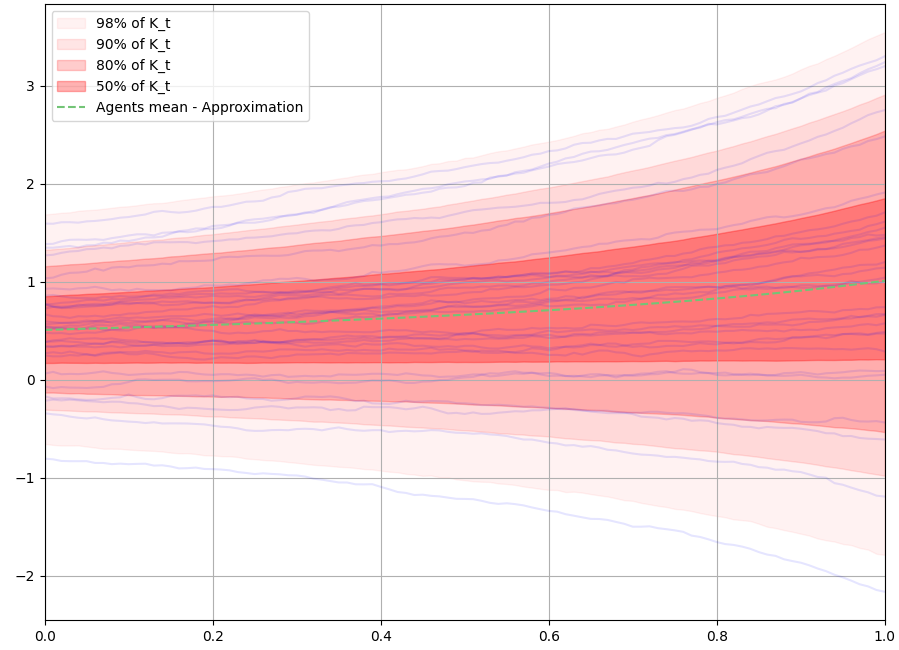
\includegraphics[width=\textwidth]{presentation/population_measure_flow_upper.png}
\caption[Economic Growth Model Population Measure Flow]{Population measure flow at the Nash equilibrium.}
\label{economicGrowthModel:populationMeasureFlow}
\end{figure}

\end{frame}
\if{
\section{Theoretical Review}

\begin{frame}{Theoretical Review - Overview}
\begin{itemize}
    \item Theoretical background:
    \begin{itemize}
        \item Stochastic optimal control
        \item Wasserstein spaces
        \item Example of Convergence of $N$-player game to MFG system
    \end{itemize}
\end{itemize}
\end{frame}

\begin{frame}{Theoretical Review - Stochastic Optimal Control}
\begin{itemize}
    \item Controlled stochastic differential equation:
    \begin{equation}
        d X_s = b(X_s, \alpha_s)ds + \sigma(X_s, \alpha_s) d W_s
    \end{equation}
    \item Objective function:
    \begin{equation}
        J(t, x, \alpha) = \mathbb{E}\left[ \int_t^T f(s, X_s^{t,x}, \alpha_s) ds + g(X^{t,x}_T) \right]
    \end{equation}
    \item Value function:
    \begin{equation}
        v(t,x) = \sup_{\alpha \in \mathcal{A}(t,x)} J(t,x,\alpha)
    \end{equation}
\end{itemize}
\end{frame}

\begin{frame}{Theoretical Review - Dynamic Programming Principle}
\begin{theorem}[Dynamic Programming Principle]
    The value function $v$ satisfies:
    \begin{gather} 
        v(t,x) = \sup_{\alpha \in \mathcal{A}(t,x)}
        \sup_{\theta \in \mathcal{T}_{t,T}}
        \mathbb{E}\left[ \int_t^\theta f(s, X_s^{t,x}, \alpha_s) ds + v(\theta, X^{t,x}_\theta) \right]
    \end{gather}
    where $\mathcal{T}_{t, T}$ is the set of stopping times valued in $[t,T]$.
\end{theorem}

\begin{itemize}
    \item Leads to the Hamilton-Jacobi-Bellman (HJB) equation:
    \begin{equation}
        -\frac{\partial v}{\partial t} - H(t,x,\partial_x v, \partial_{xx} v) = 0
    \end{equation}
    \item Terminal condition: $v(T,x) = g(x)$
\end{itemize}
\end{frame}

\begin{frame}{Theoretical Review - Viscosity Solutions}

    \begin{itemize}
        \item To derive HJB equation from DPP, we assume smoothness of the Value function. This does not necessarily hold - \highlight{HJB might not have a classical solution.}
        \item \highlight{Viscosity solutions} are weak solutions for PDEs - relaxing the smoothness assumption. 
        \item uniqueness can be proved through comparison principles.
        \item Originally defined as the unique limit $u$ as $\epsilon \to 0^+$ of solutions $u^\epsilon$ to
        \begin{equation*}
        F(x, u^\epsilon, D u^\epsilon) = \epsilon \Delta u^\epsilon
        \end{equation*}
        \item Equivalent definitions can be given in terms of test functions or sup/sub-differential sets. 
        \item We refer to \cite{pham2009continuous,bressan2007introduction,lopes1997introduccao,crandall1992user} for a thorough exposition of the topic.
        
    \end{itemize}

    
\end{frame}

\begin{frame}{Theoretical Review - Viscosity Solutions}
\begin{definition}[Second Order Viscosity Solutions]
    \begin{itemize}
        \item A function $u$ is a viscosity subsolution if
        $F(x_0, u(x_0), D \phi(x_0), D^2 \phi(x_0)) \leq 0$
        for all test functions $\phi$ at maximum points of $u - \phi$
        
        \item A function $u$ is a viscosity supersolution if
        $F(x_0, u(x_0), D\phi(x_0), D^2 \phi(x_0)) \geq 0$
        for all test functions $\phi$ at minimum points of $u - \phi$
        
        \item A function $u$ is a viscosity solution if it is both a subsolution and a supersolution
    \end{itemize}
\end{definition}

\end{frame}

\begin{frame}{Theoretical Review - Wasserstein Spaces}
    \begin{itemize}
        \item Metric space over the set of probability measures $\mathcal{P}(\Omega)$ over $\Omega \subset \RR^n$.
        \item Wasserstein distance $d_2(\mu, \nu)$for $(\mu, \nu)$ defined as the minimum quadratic cost for mass transport from $\mu \to \nu$
        \item Absolutely continuous curves over Wasserstein space described by solutions to transport equation. This means that $d_2$ is \textit{compatible } with displacement of mass by vector fields.
        \item One important property - $d_2$ does not allow for mass to "teleport" 
    \end{itemize}
\end{frame}

\begin{frame}{Theoretical Review - Wasserstein Spaces}

    \begin{itemize}
        \item Let $\Omega \subset \RR^n$, $\mathcal{P}(\Omega)$ be the set of Borel
probability measures on $\Omega$, and $\mathcal{P}_2(\Omega) \subset \mathcal{P}(\Omega)$
be the set of probability measures $m$ such that $\int_\Omega |x|^2 dm(x) < + \infty$.

        \item We can define a metric over $\mathcal{P}_2(\Omega)$ called the 
\textit{Wasserstein distance} by
\begin{equation}\label{prob_measures:wasserstein_distance}
    d_2(\mu, \nu) = \inf_{\gamma \in \Pi(\mu,\nu)} {\left[ \int_\Omega |x - y|^2 d\gamma(x,y) \right]}^{\frac{1}{2}}
\end{equation}
where $\Pi(\mu,\nu)$ is the \textit{coupling} between $\mu$  and $\nu$,
that is, the set of Borel probability measures on $\Omega \times \Omega$
such that $\gamma(A \times \Omega) = \mu(A)$ and $\gamma(\Omega \times A) = \nu(A)$
for any Borel set $A \subset \Omega$.
\item We refer to ~\cite{cardaliaguet2010notes,ambrosio2005gradient,ambrosio2021lectures} for a thorough exposition of the topic.
\end{itemize}

\end{frame}



\begin{frame}{Theoretical Review - Wasserstein Spaces}

\begin{definition}[Absolutely Continuous Curves in Wasserstein space]\label{wass:absolutely_continuous_curves}
    Let $v : (a,b) \mapsto \mathcal{P}_2(\Omega)$ be a curve.
    We say that $v$ is absolutely continuous if there exists
    $m \in L^1(a,b)$ such that
    \begin{equation}\label{wass:absolute_continuity}
        d(v(s), v(t)) \leq \int_s^t m(r) dr, \forall a < s \leq t < b.
    \end{equation}
\end{definition}

Among all choices of $m$ in~\eqref{wass:absolute_continuity}, there is a minimal
one, which describes the \textit{metric derivative} of the curve.
\end{frame}

\begin{frame}{Theoretical Review - Wasserstein Spaces}

\begin{theorem}[Absolutely continuous curves and the continuity equation]\label{wass:abs_continuity_and_continuity_eq}
    Let $\mu_t : (a,b) \mapsto \mathcal{P}_2(\Omega)$ be an absolutely continuous
    curve and let $|\mu'| \in L^1(a,b)$ be its metric derivative.
    Then there exists a Borel vector field $v : (x,t) \mapsto v_t(x)$ such that
    \begin{equation}
        v_t \in L^2(\mu_t, \Omega), ||v_t||_{L^2(\mu_t, \Omega)} \leq |\mu'|(t)\text{ for a.e. } t \in (a,b)
    \end{equation}
    and $\mu_t$ is a weak solution to the continuity equation
    \begin{equation}
        \partial_t \mu_t + \nabla \cdot (v_t \mu_t) = 0.
    \end{equation}
    Conversely, if a a curve which is continuous w.r.t.~the narrow topology
    $\mu_t : (a,b) \mapsto \mathcal{P}_2(\Omega)$
    satisfies the continuity equation for some Borel velocity field $v_t$ with
    $||v_t||_{L^1(\mu_t, \Omega)} \in L^1(a,b)$ then $\mu_t$ is absolutely continuous
    and $ |\mu'|(t) \leq  ||v_t||_{L^1(\mu_t, \Omega)}$ for a.e. $t \in (a,b)$.
\end{theorem}

\end{frame}

\begin{frame}{Theoretical Review - Wasserstein Spaces}
    \begin{theorem}[Benamou-Brenier Formula]
    For all  $\mu_0, \mu_1 \in \mathcal{P}_2(\Omega)$, we have
    \begin{align*}
        d_2(\mu_0, & \mu_1) =  \\  \min &\left\{ \int_0^1 ||v_t||^2_{L^2(\mu_t, \Omega)} \, dt : \partial_t \mu_t + \nabla \cdot (v_t \mu_t) = 0 \text{ in } (0,1) \times \Omega \right\}
    \end{align*} 
    where the minimization is among all curves $\mu_t : [0,1] \mapsto \mathcal{P}_2(\Omega)$
    continuous w.r.t.~the weak topology.
\end{theorem}

Benamou-Brenier Formula implies that,
for each pair of measures $\mu, \nu \in \mathcal{P}_2(\Omega)$,
there exists an absolute continuous curve $\mu^*_t$ starting at $\mu$ and ending at $\nu$ 
(which we call the \textit{geodesic curve})
such that $\mu^*_t$ is driven by a vector field $v_t$, and the quadratic action
$\int_0^1 ||v_t||^2_{L^2(\mu_t, \Omega)} \, dt$ of $v_t$
is both minimal and realizes the Wasserstein distance.
\end{frame}
%Our goal is to characterize absolute continuous measure flows as solutions to the continuity equation,
%and to define the derivative of function in Wasserstein space with respect to the measure.
\begin{frame}{Theoretical Review - Lyons Derivative}
\begin{itemize}
    \item In the theory of mean-field games, it is convenient to define some
form of differentiability for functions
 $\mathcal{U} : \mathcal{P}_2(\Omega) \mapsto \RR$ of probability measures.
 \item This is not straightforward to do, as the Wasserstein space lacks a vector space
 structure.
\item There are at least three aproaches to define derivatives $D_m U$ of functions in
Wassertein spaces: 
\begin{itemize}
    \item ~\cite{ambrosio2005gradient} defines a kind of manifold structure
on the Wasserstein space;
\item ~\cite{cardaliaguet2019master} restricts the 
function $U$ to elements of $\mathcal{P}_2(\Omega)$ which have a density in 
$L^2(\Omega)$ to use its Hilbert structure; 
\item ~\cite{cardaliaguet2010notes} introduces a ``lifted'' function $\tilde u$ over the space of $L^2$ random variables with values
in $\Omega$ such that $\tilde u(X) = U(\mathcal{L}(X))$, and uses the Hilbert structure
of the space of $L^2$ random variables.
\end{itemize}
\item ~\cite[Ch 5]{carmona2018probabilistic} shows that the three notions are equivalent.
\end{itemize}

\end{frame}

\begin{frame}{Theoretical Review - Lyons Derivative}
 One property of the derivative $D_m U$ is that it satisfies a form of chain rule with respect to absolute continuous flows of measures. We adopt this property as definition, for it satisfies our needs.

\begin{definition}
We say that a function $U : \mathcal{P}_2(\Omega) \mapsto \RR$ is differentiable 
at $\mu$ if there exists an element $D_m(\mu, \cdot) \in L^2_\mu$
such that for every vector field $v_t$, if we let $\mu_t$ be the solution 
to $\partial_t \mu_t + \nabla \cdot(v_t \mu_t) = 0, \mu_0 = \mu$
it follows that
\begin{equation}\label{wass:measure_derivative_chain_rule}
    \frac{d}{dt} U{(\mu_t)}_{t = 0} = \int_\Omega D_m U(\mu, y) \cdot v_0(y) d\, \mu(y)
\end{equation}
We say that $U$ is $C^1$ in a neighborhood of $\mu$ if there is a neighborhood of $\mu$ where it is differentiable.
\end{definition}
\end{frame}

\begin{frame}{Theoretical Review - $N$-Player Game Convergence Example}
    We follow~\cite{cardaliaguet2010notes} to give an example of mean field convergence in the number of players.
Consider a game with $N$ players in $\RR^d$ Each player
controls his velocity. The state of player $i$ evolves according to
\begin{equation}
    dx_i(t) = \alpha_i(t)\, dt.
\end{equation}
The cost functional for player $i$ is of the form
\begin{equation}
    J_i(x, t, {(\alpha_j)}_j) = \int_t^T L_i (x_1(s), \dots, x_N(s), \alpha_i(s)) ds + g_i(x_1(T), \dots, x_N(T))
\end{equation}

Let $\delta_x$ be the Dirac measure at point $x$. Then, We assume that
\begin{equation}
    L_i(x_1, \dots, x_N, \alpha) = \frac{1}{2}|\alpha|^2 + F\left( \frac{1}{N-1} \sum_{j \neq i} \delta_{x_j}  \right)
\end{equation}
where $F : \mathcal{P}_2 \mapsto \RR$ is continuous, and
\begin{equation}
    g_i(x_1, \dots, x_N) = g(x_i, \frac{1}{N-1} \sum_{j\neq i} \delta_{x_j})
\end{equation}
where $g: \RR^d \times \mathcal{P}_2$ is continuous.
\end{frame}

\begin{frame}{Theoretical Review - $N$-Player Game Convergence Example}

We also assume that a smooth, symmetric Nash equilibrium in feedback form exists for
this game - that is, there is a value function
$U^N : \RR^d \times [0,T] \times {(\RR^d)i}^{(N-1)} \mapsto \RR$ such that
the value function for player $i$ $U^N_i$ satisfies
\begin{equation}
    U^N_i(x_i, t, {(x_j)}_{j\neq i}) = U^N(x_i, t, {(x_j)}_{j\neq i})
\end{equation}
and the system of HJ equations
\begin{equation}
    -\partial_t U_i^N + \frac{1}{2}|\partial_{x_i} U_i^N|^2 - F\left( \frac{1}{N-1}  \sum_{j\neq i} \delta_{x_j} \right) + \sum_{j \neq i} \langle \partial_{x_j} U^N_j, \partial_{x_j} U^N_i \rangle = 0
\end{equation}
is satisfied. 
\begin{proposition}
The family of feedbacks $({\bar\alpha}_i(x,t) = - \partial_{x_i} U^N_i (x,t))$
provides a Nash equilibrium for the game.
\end{proposition}

\end{frame}

\begin{frame}{Theoretical Review - $N$-Player Game Convergence Example}

Now, assume that $U^N$ satisfy the following estimates
\begin{equation}
    \sup_{x_1, t, {(x_j)}_{j \geq 2}} \left| \partial_{x_1} U^N (x_1, t, {(x_j)}_{j \geq 2}) \right| \leq C,
\end{equation}
and
\begin{equation}
    \sup_{x_1, t, {(x_j)}_{j \geq 2}} \left| \partial_{x_j} U^N (x_1, t, {(x_j)}_{j \geq 2}) \right| \leq  \frac{C}{N}.
\end{equation}
Under these conditions, and up to a subsequence, there is a map 
$U : \RR^d \times [0,T] \times \mathcal{P}_2 \mapsto \RR$ such that,
for any $R > 0$,
\begin{equation}
    \sup_{|x| \leq R, t, {(x_j)}_{j\geq 2}} | U^N(x,t,m^{N-1}_{(x_j)}) - U(x,t,m^N_x) | \to 0\text{ as } N \to \infty,
\end{equation}
where
\begin{equation}
    m^{N-1}_{(x_j)} = \frac{1}{N-1} \sum_{j \geq 2} \delta_{x_j}, \text{ and } m^N_x = \frac{1}{N} \sum_{j = 1}^N \delta_{x_j}.
\end{equation}

\end{frame}


\begin{frame}{Theoretical Review - $N$-Player Game Convergence Example}
We also have convergence of the derivatives
\begin{equation}
    \frac{\partial U^N}{\partial t} \to \frac{\partial U(x,t,m)}{\partial t}, \quad |\partial_{x_i} U^N|^2 \to |\partial_x U (x,t,m)|^2.
\end{equation}
Finally, the sum of the inner products converges to the derivative with respect to the limit measure $m$
\begin{equation}
    \sum_{j\neq i} \langle \partial_{x_j} U^N_i , \partial_{x_j} U^N_j \rangle \to \langle D_m U(x,t,m), \partial_x U(x, t, m) \rangle_{L^2_m}.
\end{equation}
\end{frame}

\begin{frame}{Theoretical Review - $N$-Player Game Convergence Example}
    From these convergence results, we have that the limit of $U^N$ as $N \to \infty$
is some $U\in \mathcal{C}^0(\RR^d \times [0,T] \times \mathcal{P}_2) $
 which satisfies 
 \begin{equation}\label{wass:simple_master_equation}
    \begin{cases}
        - \frac{\partial U}{ \partial t} + \frac{1}{2} |\partial_x U(x,t,m)|^2 - F + \langle D_m U, \partial_x U \rangle_{L^2_m} = 0 \\\text{ in }\RR^d \times [0,T] \times \mathcal{P}_2,\\
        U(x,T,m) = g(x,m)
    \end{cases}
 \end{equation}
 Note that this differential equation includes a differential with respect to
 a probability measure.

 
  Let us apply an idea similar to the method of characteristics to this equation:

\end{frame}

\begin{frame}{Theoretical Review - $N$-Player Game Convergence Example}
      Let $m(t)$ be an absolute continuous measure flow over $\mathcal{P}_2$, and
  let $u(x,t) = U(x,t,m(t))$. We have, by the chain rule of the Lyons derivative:
\begin{equation}
    \frac{\partial u}{\partial t} = \frac{\partial U}{\partial t} + \langle D_m U (\cdot, t, m(t)), v(t) \rangle_{L^2_{m(t)}},
\end{equation}
    where $v(t)$ is the vector field driving $m(t)$ through the continuity equation $\partial_t m + \nabla \cdot( m(x,t) v(x,t) ) = 0$.
    We can rewrite equation~\eqref{wass:simple_master_equation} as 
\begin{equation}
    \frac{\partial U}{ \partial t} + \langle D_m U, - \partial_x U \rangle_{L^2_m} = \frac{1}{2} |\partial_x U(x,t,m)|^2 - F.
\end{equation}

\end{frame}

\begin{frame}{Theoretical Review - $N$-Player Game Convergence Example}
        Therefore, if we \textit{choose} as driver of $m(t)$ the vector field 
\begin{equation*}
    v(x,t) = - \partial_x U(x,t,m(t)) = - \partial_x u(x,t),
\end{equation*}
    we have
\begin{align*}
    \frac{\partial u}{\partial t} &=  \frac{\partial U}{ \partial t}(x,t,m(t)) + \langle D_m U(\cdot, t, m(t) ), - \partial_x U(\cdot, t, m(t) ) \rangle_{L^2_m}\\
    &= \frac{1}{2} |\partial_x u(x,t)|^2 - F
\end{align*}
    from which we arrive at the MFG system of PDEs:
\begin{equation}
    \begin{cases}
        - \frac{\partial u}{\partial t} + \frac{1}{2} |\partial_x u(x,t)|^2  = F(m), \\
        \partial_t m - \nabla \cdot( \partial_x u(x,t) m(x,t) ) = 0,\\
        m(0) = m_0, \, u(x,T) = g(x, m(T))
    \end{cases}
\end{equation}
    where the first equation holds in the viscosity sense, and the second
    one holds in the sense of distributions.
    The vector field $v(x,t) = -\partial_x U(x,t,m(t))$ is aptly called the \textit{decoupling field}.
\end{frame}

}\fi
\section{Proposed Model}

\begin{frame}{Proposed Model - Model Introduction}
\begin{itemize}
    \item Game theoretical model for time allocation between work and education
    \item Based on Lucas's human capital growth model\footnote{~\cite{lucas1988mechanics}} and Aiyagari's growth model\footnote{ ~\cite{achdou2014partial}}
    \item Interactions through interest rate and wage rate
    \item Motivated by high rate of school evasion in Brazil due to necessity of working
    \begin{itemize}
        \item 45\% of people out of school (15-29 years old) cite work needs as reason for not pursuing education\footnote{~\cite{pnad2023short}}
    \end{itemize}
    \item Expected outcomes:
    \begin{itemize}
        \item Qualitative properties of population behavior
        \item Numerical solutions of the mean field limit
        \item Modeling public policies to promote education
    \end{itemize}
\end{itemize}
\end{frame}

\begin{frame}{Proposed Model - Model Description}
\begin{itemize}
    \item $N$ agents with wealth $A_t$ and skill level $H_t$
    \item Controls: consumption $c_t$ and proportion of time dedicated to working $u_t$
    \item Proportion $1-u_t$ used for improving skill level
    \item Optimization problem:
    \begin{equation}
    \begin{cases}
        \sup\limits_{(u,c) \in \mathcal{U} \times \mathcal{C}}\mathbb{E} [ \int_0^T f_c(c^i_s) + f_u(u^i_s) ds + Q(A^i_T) ]\\
        d A^i_t = \left[ (\bar r_t - \delta) A^i_t + \bar w_t H^i_t u^i_t - c^i_t  \right] dt + \sigma_a A^i_t d W^{a,i}_t\\
        d H^i_t = (H^i_t)^\xi g(1 - u^i_t) dt + \sigma_h H^i_t d W^{h,i}_t
    \end{cases}
    \end{equation}
\end{itemize}
\end{frame}

\begin{frame}{Proposed Model - Wealth and Skill Dynamics}
\begin{itemize}
    \item Wealth dynamics:
    \begin{itemize}
        \item Interest returns: $(\bar r_t - \delta) A_t$
        \item Wages: $\bar w_t H_t u_t$ (proportional to time and skill)
        \item Consumption: $-c_t$
        \item Noise term: $\sigma_a A_t d W^a_t$
    \end{itemize}
    \item Skill dynamics:
    \begin{itemize}
        \item Skill improvement: $H^\xi_t g(1 - u_t)$
        \item Parameter $\xi$ captures impact of current skill on effectiveness
        \item Noise term: $\sigma_h H_t dW^h_t$
    \end{itemize}
\end{itemize}
\end{frame}

\begin{frame}{Proposed Model - Mean Field Interactions}
\begin{itemize}
    \item Interaction through $\bar r_t$ and $\bar w_t$
    \item Cobb-Douglas production function $F$ depending on:
    \begin{itemize}
        \item Average wealth 
        $$\bar a(\mu_t) \coloneqq \int_\Omega \, a \, d\mu_t (a,h)$$
        \item Effective supply of skilled labor 
        $$\heff(\mu_t) \coloneqq \int_\Omega \, u(a,h) h \, d\mu_t (a,h)$$
    \end{itemize}
    \item Agents distributed with measure $\mu^N_t \in \mathcal{P}(\Omega)$
    \item At economic equilibrium:
    \begin{align}
        \bar r(\mu^N_t) &= \partial_a F(\bar a(\mu^N_t), \heff(\mu^N_t))\\
        \bar w(\mu^N_t) &= \partial_h F(\bar a(\mu^N_t), \heff(\mu^N_t))
    \end{align}
\end{itemize}
\end{frame}

\begin{frame}{Proposed Model - Analytic Formulation}
The MFG PDE system is given by:
\begin{equation}
    \begin{cases}
        \partial_t V + (\bar r  - \delta) a \partial_a V + \HH_u(h, \partial_a V, \partial_h V)  + \HH_c(\partial_a V) \\
        \quad\quad + \frac{1}{2} \sigma_a^2 a^2 \partial_{aa} V + \frac{1}{2} \sigma^2_h h^2 \partial_{hh} V = 0,\\[10pt]
        \partial_t \mu + \partial_a \left( \left[ (\bar r - \delta) a + \partial_p \HH_u(h, \partial_a V, \partial_h V) + \partial_p \HH_c(\partial_a V) \right] \mu \right) \\
        \quad\quad + \partial_h \left( \partial_q \HH_u(h, \partial_a V, \partial_h V)\, \mu\right) \\
        \quad\quad - \frac{1}{2} \sigma_a^2 \partial_{aa} (a^2\mu) - \frac{1}{2} \sigma^2_h \partial_{hh} (h^2\mu) = 0,\\[10pt]
        \mu(0,a,h) = \mu_0,\quad V(T,a,h) = Q(a)
    \end{cases}
\end{equation}

where $\HH_u$ and $\HH_c$ are Hamiltonian functions for the optimization problems
\end{frame}

\begin{frame}{Proposed Model - MV-FBSDE Formulation}
Alternative formulation with Forward-Backward SDEs:
\begin{equation}
    \begin{cases}
        d A_t = \left[ (\bar r_t - \delta) A_t + \bar w_t H_t {\hat u}_t - {\hat c}_t  \right] dt + \sigma_a A_t d W^a_t,\\
        d H_t = H^\xi_t g(1 - {\hat u}_t) dt + \sigma_h H_t d W^h_t,\\
        d P_t = -\left[ (\bar r_t - \delta) P_t + \sigma_a Z^p_t \right]dt + Z^p_t d W^a_t,\\
        d Q_t = - \left[ \xi H_t^{\xi - 1} g(1 - {\hat u}_t ) Q_t + {\bar w} {\hat u}_t P_t + \sigma_h Z^q_t \right] dt + Z^q_t d W^h_t,\\
        \mathcal{L}(A_0, H_0) = \mu_0, \, P_T = \partial_a Q(A_T), Q_T = 0
    \end{cases}
\end{equation}

With $\hat u_t \coloneqq \hat u(H_t,P_t,Q_t)$ and $\hat c_t \coloneqq \hat c(P_t)$
\end{frame}

\begin{frame}{Proposed Model - Numerical Illustration}
\begin{itemize}
    \item $N$-player deterministic version simulated through adapted shooting algorithm
    \item Simplified model:
    \begin{itemize}
        \item $g(1- u) = (1 - u)$, $\xi = 0$, $\delta = 0.05$, $k = 0.5$
        \item $f_c(c) = \log(c)$, $f_u(u) = -\frac{\alpha}{2} u^2$, $Q(a) = a$
    \end{itemize}
    \item Two scenarios: $\alpha = 0.5$ vs $\alpha = 2$ (lower vs higher preference for education)
\end{itemize}
\end{frame}

\begin{frame}{Proposed Model - Numerical Illustration - States}

\begin{figure}[h!]
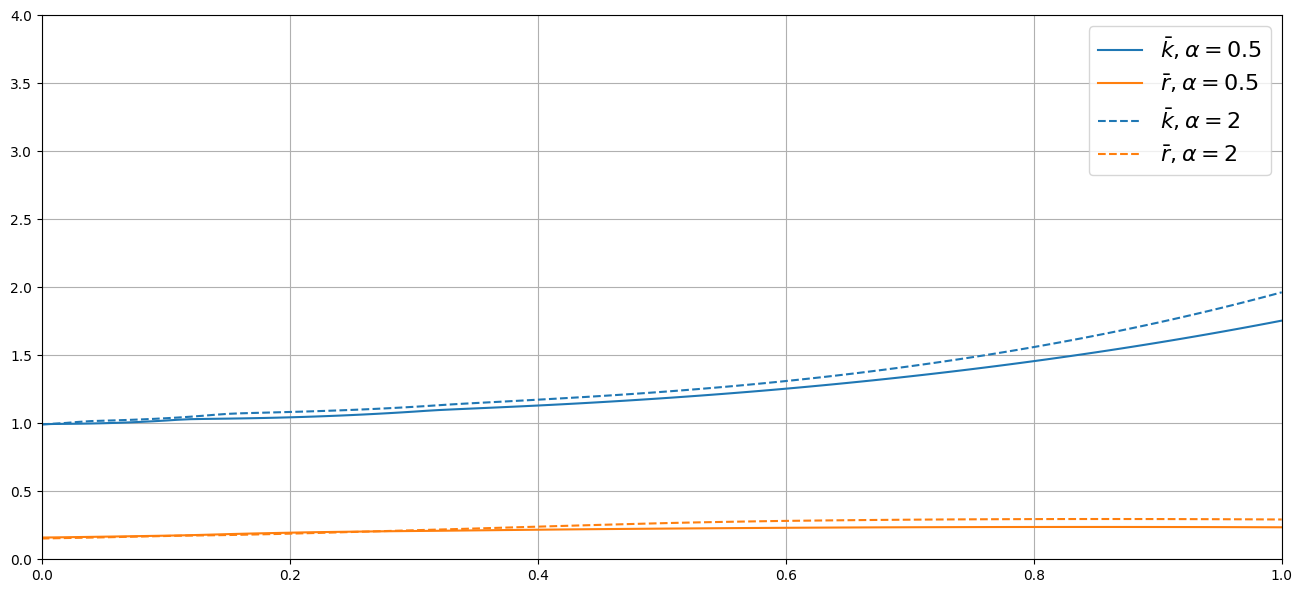
\includegraphics[width=\textwidth]{presentation/model_simulations/simulations_mfg_states.png}
\end{figure}
\end{frame}


\begin{frame}{Proposed Model - Numerical Illustration - Controls}
\begin{figure}[h!]
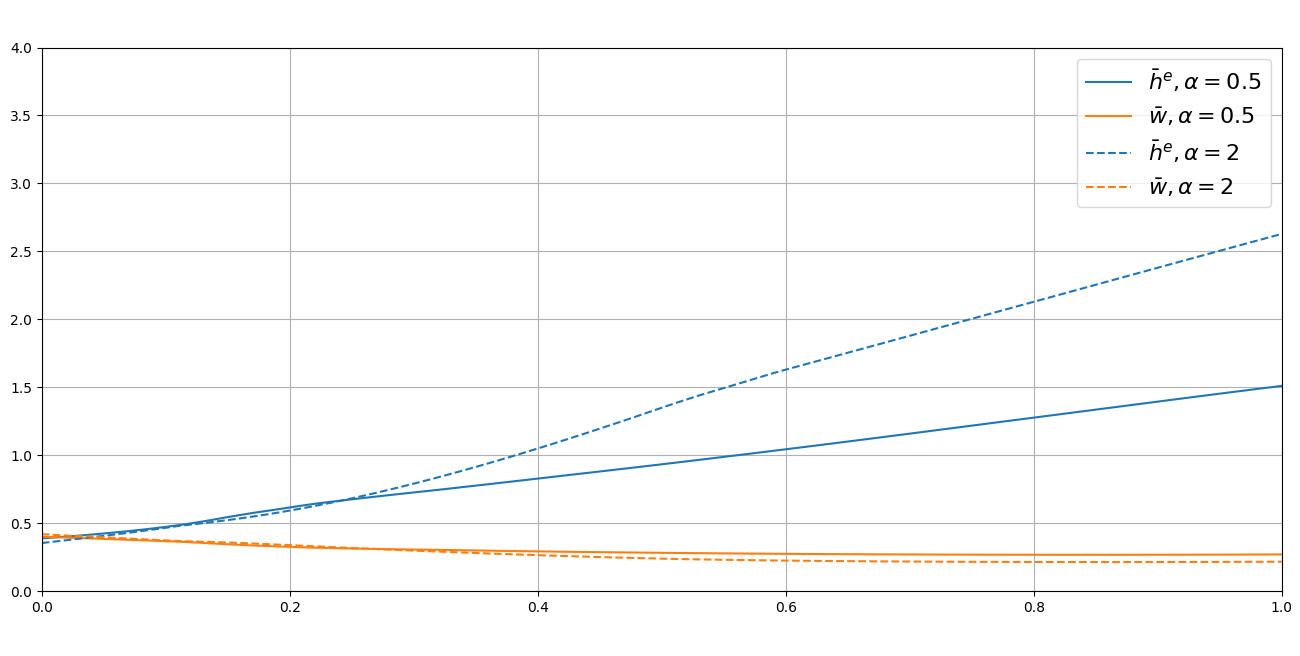
\includegraphics[width=\textwidth]{presentation/model_simulations/simulations_mfg_controls.png}
\end{figure}

\end{frame}


\begin{frame}{Proposed Model - Numerical Illustration - Production Function}
\begin{figure}[h!]
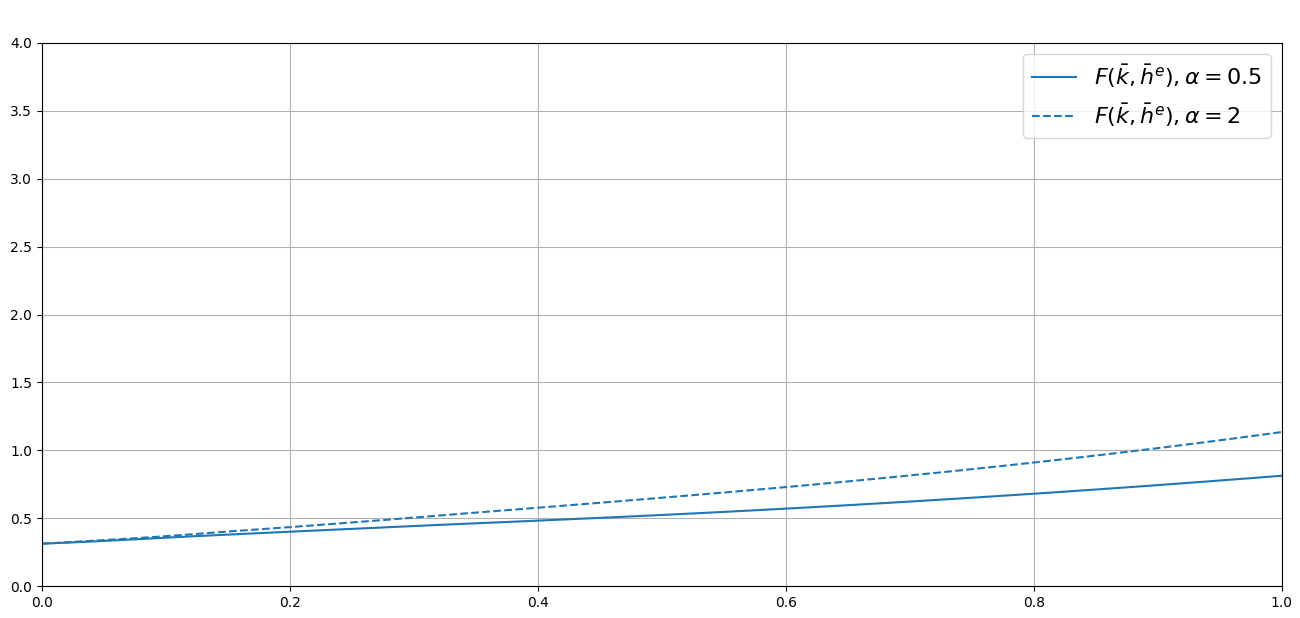
\includegraphics[width=\textwidth]{presentation/model_simulations/simulations_mfg_production.png}
\end{figure}

\end{frame}

\begin{frame}{Simulation Results}
\begin{itemize}
    \item Increased preference for education leads to:
    \begin{itemize}
        \item Increased average wealth
        \item Higher interest rates
        \item Higher aggregate production
        \item Effective supply of skilled labor:
        \begin{itemize}
            \item Decrease in the short term
            \item Increase in the long term
        \end{itemize}
        \item Decreased wages per skill per time
    \end{itemize}
\end{itemize}
\end{frame}

\section{Conclusion}

\begin{frame}{Conclusion and Future Work}
\begin{itemize}
    \item Reviewed mean field game theory
    \item Proposed a model of effects of education preferences on the economy
    \item Next steps:
    \begin{itemize}
        \item Simulate full model using deep neural networks
        \item Derive analytical results for the model
        \item Propose modifications to the baseline model
        \item Consider principal-agent mean field control problem:
        \begin{itemize}
            \item Decision maker optimizing public policy
            \item Associated utility over population distribution state
        \end{itemize}
    \end{itemize}
\end{itemize}
\end{frame}

\begin{frame}{Summary}
\begin{itemize}
    \item Mean Field Games provide a powerful framework for studying strategic interactions in large populations
    \item Educational choice model:
    \begin{itemize}
        \item Captures trade-off between work and education
        \item Shows how individual preferences affect aggregate outcomes
        \item Demonstrates the economic benefits of education
    \end{itemize}
    \item Applications:
    \begin{itemize}
        \item Educational policy design
        \item Understanding wealth and skill distribution dynamics
        \item Predicting economic impacts of educational incentives
    \end{itemize}
\end{itemize}
\end{frame}

\begin{frame}[allowframebreaks]{References}
\tiny{\printbibliography}
\end{frame}

\end{document}